\subsubsection{Spatial Sort}
\label{sec:optim:sort}

Traversing an irregular structure requires loading from memory the elements of the structure which, due to their irregular nature, can not be obtained in a optimized way through prefetching. Also due to their irregular nature, the elements of this structure which are consecutively accessed (especially in parallel) will most probably lie in distinct cache lines, hurting locality.

By changing the order of accesses in these structures, so that domain objects with similar traverse patterns become consecutive, temporal locality is improved as the elements a given object will touch are already likely to have been touched by the previous one.

Sorting these objects in a abstract space can be performed using space-filling curves\footnote{A curve which touches every object in the domain only once. Examples of these curves are the Peano and Hilbert curves.}. The examples described in this document use the CGAL library, implementing the traits required for spatial sorting in 3D.

\begin{figure}[!htp]
	\centering
	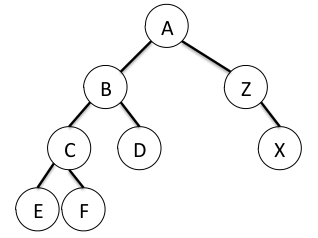
\includegraphics[width=0.4\columnwidth]{pointblocking_tree}
	\caption{A sample tree}
	\label{fig:tree}
\end{figure}

\begin{figure}[!htp]
	\centering
	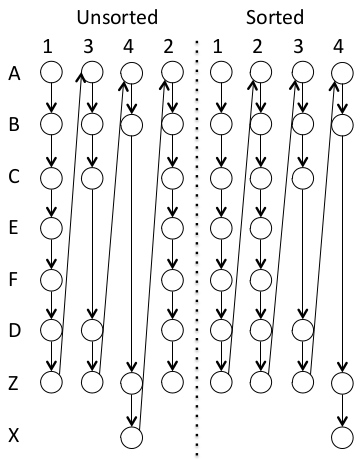
\includegraphics[width=0.6\columnwidth]{pointblocking_sort}
	\caption{Spatial Sort transformation applied to traversal of tree shown in \cref{fig:tree}}
	\label{fig:sort}
\end{figure}

\paragraph{Limitations:}
Processing the points by their geometrical position is only enough with smaller traversal sizes, where the entire traversal fits in cache, and subsequent points, which are likely to follow similar paths due to being geometrically close, will benefit from locality.

But for a sufficiently large traversal, the first visited nodes will have been evicted from cache at the end of the traversal, and when starting the next traversal, will have to be fetched again, increasing misses. \cite{tree_tiler} already shows that, as the traversao size increases, the locality improvements gained from the spatial sort optimization decrease drastically.